\documentclass[10pt]{beamer}

% This file is a solution template for:

% - Giving a talk on some subject.
% - The talk is between 15min and 45min long.
% - Style is ornate.

\usepackage[T1]{fontenc}
\usepackage[utf8]{inputenc}
\usepackage[slovene]{babel}
\usepackage{lmodern} 
\usepackage{graphicx}

\setbeamertemplate{navigation symbols}{}
\setbeamertemplate{frame number}{}                                                                                         

\setbeamerfont{caption}{size=\tiny}
\setbeamercolor{caption name}{fg=black}

\setbeamertemplate{caption}{\raggedright\centering\insertcaption\par}

\usepackage{ragged2e}
\usepackage{comment}

\usepackage{algorithm2e}
\usepackage{algpseudocode}
\SetKwInOut{KwIn}{Vhod}
\SetKwInOut{KwOut}{Izhod}
\SetAlgorithmName{Algoritem}

% Copyright 2004 by Till Tantau <tantau@users.sourceforge.net>.
%
% In principle, this file can be redistributed and/or modified under
% the terms of the GNU Public License, version 2.
%
% However, this file is supposed to be a template to be modified
% for your own needs. For this reason, if you use this file as a
% template and not specifically distribute it as part of a another
% package/program, I grant the extra permission to freely copy and
% modify this file as you see fit and even to delete this copyright
% notice. 


\mode<presentation>
{
  \usetheme{Copenhagen}
  % or ...
  \usecolortheme{seahorse}
  % \setbeamercovered{transparent}
  % or whatever (possibly just delete it)
}

% Or whatever. Note that the encoding and the font should match. If T1
% does not look nice, try deleting the line with the fontenc.

\newcommand{\bx}{\mathbf{x}}
\DeclareMathOperator{\Gl}{Gl}
\DeclareMathOperator{\adj}{adj}
%\newcommand{\Gl}{{\mathrm {GL}}\,}
\newtheorem{proposition}[theorem]{Proposition}

\theoremstyle{definition}
\newtheorem{defin}{Definicija}
\newtheorem{izrek}[defin]{Izrek}
\newtheorem{primer}[defin]{Primer}
\newtheorem{trditev}[defin]{Trditev}


\title[Diplomski seminar] % (optional, use only with long paper titles)
{Bernstainovi baznih polinomov treh spremenljivk}

%\subtitle
%{Kratka predstavitev teme} % (optional)

\author[Lina Ivanova, Tia Krofel] % (optional, use only with lots of authors)
{Lina Ivanova, Tia Krofel
\newline
\newline
\newline 
}

% - Use the \inst{?} command only if the authors have different
%   affiliation.
%  \institute[FMF] % (optional, but mostly needed)
%  {
%    \inst{}%
%    Finančna matematika - 1. stopnja
%  \and
%  \inst{2}%
%  Department of Theoretical Philosophy\\
%  University of Elsewhere
%  }
% - Use the \inst command only if there are several affiliations.
% - Keep it simple, no one is interested in your street address.

\date[13. januar  2023] % (optional)
{13. januar  2023}

% \subject{Talks}
% This is only inserted into the PDF information catalog. Can be left
% out. 



% If you have a file called "university-logo-filename.xxx", where xxx
% is a graphic format that can be processed by latex or pdflatex,
% resp., then you can add a logo as follows:

% \pgfdeclareimage[height=0.5cm]{university-logo}{university-logo-filename}
% \logo{\pgfuseimage{university-logo}}



% Delete this, if you do not want the table of contents to pop up at
% the beginning of each subsection:
%\AtBeginSubsection[]
%{
%  \begin{frame}<beamer>
%    \frametitle{Outline}
%    \tableofcontents[currentsection,currentsubsection]
%  \end{frame}
%}


% If you wish to uncover everything in a step-wise fashion, uncomment
% the following command: 

%\beamerdefaultoverlayspecification{<+->}


\begin{document}

\begin{frame}
  \titlepage
\end{frame}

%\begin{frame}
%  \frametitle{Outline}
%  \tableofcontents
%  % You might wish to add the option [pausesections]
%\end{frame}


% Since this a solution template for a generic talk, very little can
% be said about how it should be structured. However, the talk length
% of between 15min and 45min and the theme suggest that you stick to
% the following rules:  

% - Exactly two or three sections (other than the summary).
% - At *most* three subsections per section.
% - Talk about 30s to 2min per frame. So there should be between about
%   15 and 30 frames, all told.

%\section{Determinantal Representations}

%\subsection[Definition]{Definition}

\begin{frame}

  \frametitle{Prostor $\mathbb{P}^3_n$}
  \begin{block}{}
    S $\mathbb{P}^3_n$ označimo prostor polinomov treh spremenljivk stopnje $n$, 
    torej prostor končnih dimenzij z vsemi funkcijami oblike
    $$ p(x,y,z):=\sum_{0\leq i+j+k\leq n}\alpha_{ijk}x^iy^jz^k,$$ 
    kjer $\alpha_{ijk}\in\mathbb{R}$ \pause
  \end{block}
  \vspace{0.3cm}
  Dimenzija prostora $\mathbb{P}^3_n$ je enaka $\binom{n+3}{3}$, 
  medtem ko monomi $\{x^iy^jz^k\}_{0\leq i+j+k\leq n}$ tvorijo bazo.
\end{frame}

\begin{frame}
  
  \frametitle{Baricentrične koordinate}
    Naj bo $T$ tetraeder z ogli"s"ci $\textbf{V}_{i} = (x_{i}, y_{i}, z_{i})$, kjer $i \in \{1, 2, 3, 4\}$, ozna"cen s 
    $T = \langle\textbf{V}_{1}, \textbf{V}_{2}, \textbf{V}_{3}, \textbf{V}_{4}\rangle.$
    \pause
  \begin{block}{}
    Vsako to"cko $\textbf{V} = (x, y, z) \in \mathbb{R}^{3}$  lahko na enoli"cen na"cin zapi"semo kot kombinacijo oblike
    \begin{equation*}
    \textbf{V} = u_{1}\textbf{V}_{1} + u_{2}\textbf{V}_{2} + u_{3}\textbf{V}_{3} + u_{4}\textbf{V}_{4},
    \end{equation*}
    kjer je
    $$
    u_{1} + u_{2} + u_{3} + u_{4} = 1.
    $$
  \end{block}
  \pause
  \vspace{0.2cm}
    To"cke $(u_{1}, u_{2}, u_{3}, u_{4})$ tvorijo 
    baricentri"cne koordinate neke poljubne to"cke 
    $\textbf{V} = (x, y, z)$ glede na tetraeder $T$.
    \vspace{0.2cm}
    \pause

    V nadaljevanje bomo ozna"cevali $\textbf{u} = (u_{1}, u_{2}, u_{3}, u_{4})$. 
\end{frame}

\begin{frame}
\frametitle{Domenske to"cke}

\begin{columns}

\begin{column}{0.5\textwidth}
Naj bodo $\textbf{u}$ baricentri"cne koordinate poljubne to"cke $(x, y, z)$ glede na izbran tetraeder $T = \langle\textbf{V}_{1},\textbf{V}_{2},\textbf{V}_{3}, \textbf{V}_{4}\rangle$.
\vspace{0.3cm}
Domenske to"cke Bézierjevega polinoma lahko definiramo kot
$$
\textbf{X}_{\textbf{i}} = \frac{i}{n}\textbf{V}_{1} + \frac{j}{n}\textbf{V}_{2} + \frac{k}{n}\textbf{V}_{3} + \frac{l}{n}\textbf{V}_{4}
$$
za vsak $\textbf{i} = (i, j, k, l)$, kjer $|\textbf{i}| = n$.
\end{column}

\begin{column}{0.5\textwidth}

\begin{figure}[h!]
\centering
  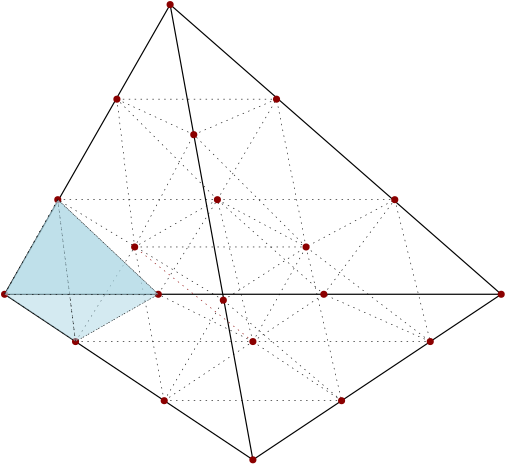
\includegraphics[scale=0.3]{domen}
  \caption{Domenske to"cke}
  \label{fig:domenske}
\end{figure}

\end{column}

\end{columns}

\end{frame}

  \begin{frame}

    \frametitle{Bernsteinovi bazni polinomi treh spremenljivk}
    Naj bo $T$ tetraeder in $u_1,u_2,u_3,u_4$
    baricentrične koordinatne funkcije.
    Potem definiramo Bernsteinov bazni polinom treh spremenljivk 
    stopnje $n$ glede na $T$ kot 
    $$
    B_{ijkl}^n(\textbf{u}) := \frac{n!}{i!\text{ }j!\text{ }k!\text{ }l!}u_1^iu_2^ju_3^ku_4^l,\text{    }i+j+k+l=n.
    $$
    \pause
    \begin{block}{}    
        Množica $\mathcal{B}^n := \{B_{ijkl}^n\}_{i+j+k+l=n}$
        Bernsteinovih baznih polinomov predstavlja bazo 
        prostora polinomov treh spremenljivk $\mathbb{P}^3_n$.\\
        \vspace{0.2cm}
        Še več,
        $
        \sum_{i+j+k+l=n}B^n_{ijkl}(\textbf{u})=1\text{ }
        $
        in

        \vspace{0.2cm}
        $
        0\leq B_{ijkl}^n(\textbf{u})\leq 1\text{ }\forall \textbf{u}=\text{Bar}{((x,y,z);T)}, (x,y,z)\in T.
        $
    \end{block}
  \end{frame}

  \begin{frame}

    \frametitle{Bernsteinovi bazni polinomi treh spremenljivk}
    \begin{itemize}
      \item Teh polinomov je $\binom{n+3}{3} = \dim{\mathbb{P}^3_n}$;\pause
      \item Tvorijo razčlenitev enote: 
      $$\sum_{|\textbf{i}|=n}B_{\textbf{i}}^n(\textbf{u})=
      \sum_{|\textbf{i}|=n}\frac{n!}{i!\text{ }j!\text{ }k!\text{ }l!}u_1^iu_2^ju_3^ku_4^l=
      (u_1+u_2+u_3+u_4)^n = 1;
      $$\pause
      \item $0\leq B_{ijkl}^n(\textbf{u})\leq 1\text{ }\forall \textbf{u}=\text{Bar}{((x,y,z);T)}, (x,y,z)\in T$;\pause
      \item Z indukcijo pokažemo še, 
      da lahko vse monome $\{x^\alpha y^\beta z^\gamma\}_{0\leq \alpha+\beta+\gamma\leq n}$ 
      zapišemo kot linearno kombinacijo Bernstainovih baznih polinomov.
    
      
    \end{itemize}
  \end{frame}


  \begin{frame}

    \frametitle{Bernsteinovi bazni polinomi treh spremenljivk}
    Pokazali smo, da $\sum_{|\textbf{i}|=n}B_{\textbf{i}}^n(\textbf{u})=1$.\pause    
    Če sedaj pomnožimo $x=u_1x_1+u_2x_2+u_3x_3+u_4x_4$ z
    $1 = \sum_{i+j+k+l=n-1}B_{ijk}^{n-1}(\textbf{u})$ in enako naredimo za 
    $y$ in $z$, dobimo:\pause

    $$
    x = \sum_{i+j+k+l=n}\frac{(ix_1+jx_2+kx_3+lx_4)}{n}B_{ijkl}^n(\textbf{u}),
    $$\pause
    $$
    y = \sum_{i+j+k+l=n}\frac{(iy_1+jy_2+ky_3+ly_4)}{n}B_{ijkl}^n(\textbf{u}),
    $$\pause
    $$
    z = \sum_{i+j+k+l=n}\frac{(iz_1+jz_2+kz_3+lz_4)}{n}B_{ijkl}^n(\textbf{u}).
    $$\pause
    Sledi $$(x,y,z) = \sum_{|\textbf{i}| = n}\bigl(\frac{i}{n}\textbf{V}_1+\frac{j}{n}\textbf{V}_2+\frac{k}{n}\textbf{V}_3+\frac{l}{n}\textbf{V}_4\bigr)B_{\textbf{i}}^n(\textbf{u})$$
\end{frame}


\begin{comment}
  \begin{frame}

    \frametitle{Bernsteinova forma polinomov treh spremenljivk}
    Vsak polinom $p \in \mathbb{P}^{3}_{n}$ lahko enolično zapišemo v obliki
    \begin{equation*} %\label{polinom}
        p(\textbf{u}) = \sum_{i + j + k + l = n}c_{ijkl}B^{n}_{ijkl}(\textbf{u}),
    \end{equation*}
    kjer so $B^{n}_{ijkl}$ Bernsteinovi baznih polinomov glede na tetraeder $T$ in $c_{ijkl}$ Bézierjevi koeficienti.
    \pause
    \vspace{0.3cm}
    \begin{block}{}
        Bézierjev tetraeder stopnje $n$, dolo"cen s kontrolnimi to"ckami $\textbf{b}_{\textbf{i}}$, $|\textbf{i}| = n$, 
        je podan s parametrizacijo
        \begin{equation*}
        \textbf{p}(\textbf{u}) = \sum_{|\textbf{i}| = n}\textbf{b}_{\textbf{i}}B_{\textbf{i}}^{n}(\textbf{u}),
        \end{equation*}
        kjer je $\textbf{u} = Bar((x, y, z); T)$.
    \end{block}

  \end{frame}
\end{comment}

\begin{frame}

\frametitle{De Casteljaujev algoritem}
 $$p(\textbf{u}) = \sum_{|\textbf{i}| = n}c_{\textbf{i}}B^{n}_{\textbf{i}}(\textbf{u})$$
 \begin{block}{}
\begin{algorithm}[H]
\caption{de Casteljaujev algoritem}
\KwIn{\textbf{$b_{\textbf{i}}$} z $|\textbf{i}| = n$, $\textbf{u} = (u_{1}, u_{2}, u_{3}, u_{4})$}
\For{\text{$r = 1, 2, \ldots, n$}}
 	{
  		\For{$|\textbf{i}| = n-r$}
		{
			$\textbf{b}^{r}_{\textbf{i}} = u_{1}\textbf{b}^{r-1}_{i+1,j,k,l} + u_{2}\textbf{b}^{r-1}_{i,j+1,k,l} + u_{3}\textbf{b}^{r-1}_{i,j,k+1,l} + u_{4}\textbf{b}^{r-1}_{i,j,k,l+1}$
		}
  	}
\KwOut{$\textbf{b}_{0,0,0,0}^{n}(\textbf{u})$}	
\vspace{4mm}
\end{algorithm}
\end{block}
\end{frame}

  \begin{frame}

    \frametitle{Odvodi}
    Če imamo podan vektor $\textbf{d} := (d_x,d_y,d_z) \in \mathbb{R}^3$ in $\textbf{v} = (x, y, z)$, 
    lahko definiramo smerne odvode funkcije treh spremenljivk $f$ kot 
    $$
    \left.D_{\textbf{d}}f(x,y,z):=\frac{d}{dt}f(x+td_x,y+td_y,z+td_z)\right|_{t=0}.
    $$
    \pause
    \begin{block}{}
        Naj bo $d \in \mathbb{R}^{3}$, 
        Bar(\textbf{d}; T) $= (\mu_1,\mu_2,\mu_3,\mu_4)$. Potem za poljubne 
        $i+j+k+l=n$ velja:

        \vspace{0.4cm}

        $$
        D_{\textbf{d}}B_{ijkl}^n(\textbf{u})=
        $$ 
        $$
        \left.\frac{d}{dt}\Bigl(\frac{n!}{i!j!k!l!}(u_{1}+t\mu_{1})^{i}(u_{2}+t\mu_{2})^{j}(u_{3}+t\mu_{3})^{k}(u_{4}+t\mu_{4})^{l}\Bigr)\right|_{t=0}=
        $$
        $$
        = n[\mu_1B_{i-1,j,k,l}^{n-1}(\textbf{u})+
        \mu_2B_{i,j-1,k,l}^{n-1}(\textbf{u})+
        \mu_3B_{i,j,k-1,l}^{n-1}(\textbf{u})+
        \mu_4B_{i,j,k,l-1}^{n-1}(\textbf{u})
        ].
        $$
        \vspace{0.4cm}
    \end{block}

  \end{frame}

\begin{comment}
  \begin{frame}
    
    \frametitle{Odvodi}
    \begin{block}{}
      Naj množica $d_1,...,d_m$ predstavlja $m$
      smeri, $\mu^{(i)}=(\mu_1^{(i)},\mu_2^{(i)},\mu_3^{(i)},\mu_4^{(i)})$ 
      pa smerne koordinate za $i = 1,...,m$. Potem velja
      enakost

      $$
      D_{d_m}\cdot ... \cdot D_{d_{1}}p(v) = \frac{n!}{(n-m)!}\sum_{i+j+k+l=n-m}
      c_{ijkl}^{(m)}(\mu^{(1)},...,\mu^{(m)})B_{ijkl}^{n-m}(v),
      $$
      \newline 
      kjer $c^{(m)}_{ijkl}(\mu^{(1)},...,\mu^{(m)})$ predstavljajo števila, ki jih 
      dobimo po izvedbi $m$ korakov de Casteljaujevega algoritma, če  
      po vrsti uporabimo vrednosti $\mu^{(1)},...,\mu^{(m)}$.
      \end{block}\pause
      \vspace{0.3cm}
      S tem izrekom se lahko še enkrat prepričamo, da 
      je $m$-ti mešani smerni odvod polinoma $p$ 
      polinom stopnje $n-m$.

  \end{frame}

\end{comment}

\end{document}
